% LTeX: language=de-DE
\chapter{Evaluation}
	Im Folgenden sollen die mechanische Integrität und Performanz des Systems in Hinblick auf die in \cref{sec:constructive limitations} formulierten Rahmenbedingungen diskutiert werden.
	Im Vorfeld wurden mehrere Testfahrten auf urbanem Untergrund und entlang verschiedener Steigungen durchgeführt.
	Insgesamt wurde die verbaute Batterie hierbei dreimal von~\qty{42}{\volt} (voll geladen) herunter auf~\qty{31}{\volt} entladen.
	Zurückgelegte Distanz und mittlere, sowie maximale Geschwindigkeit wurden mittels Navigationssoftware und GPS gemessen.
	Zusätzlich wurden Logginginformationen der ESC selbst zur Evaluation herangezogen.
	% \Cref{fig:ESC plot} zeigt den Verlauf der Geschwindigkeit in~\unit{\kilo\metre\per\hour} zusammen mit Motor- und Batteriestrom in~\unit{\percent} der jeweiligen Maximalwerte.
	Die verwendeten Parameter für Tests auf der Werkbank und im Feld können \cref{fig:ESC motor params} und \cref{fig:ESC erpm setting} entnommen werden.
	% Da aus Sicherheitsgründen einige Testläufe auf der Werkbank durchgeführt wurden und Messungen per GPS jedoch eine tatsächliche Bewegung im freien zwingend erforderlich machen, wurden zusätzlich Logginginformationen der ESC ausgelesen, um aus Umdrehungen pro Minute und Anzahl der Umdrehungen Werte zur Geschwindigkeit rechnerisch ermitteln zu können.\par\medskip
	%
	\section{Performanz}
		Während mehrerer Testfahrten wurde das Drehmoment auf einer Strecke von etwa~\qty{250}{\metre} entlang eines Hanges mit einer maximalen Steigung von~\qty{7,5}{\percent} auf gepflastertem Untergrund getestet.
		Während das System am Hang und aus dem Stand heraus nur schwer in der Lage ist zu beschleunigen, ist es ohne weiteres möglich, mit bereits moderater Anfangsgeschwindigkeit die Steigung zu überwinden.
		% \begin{figure}[h]
		% 	\centering
		% 	\includesvg[width=.85\textwidth, inkscapelatex=false]{Calc/ESC_plot}
		% 	\caption[ESC plot]{ESC plot.}%
		% 	\label{fig:ESC plot}
		% \end{figure}
		\begin{figure}[h]
			\centering
			\includesvg[width=\textwidth]{Calc/ESC_testdrive_plot}
			\caption[Aufgetragene Logging-Informationen einer Testfahrt]{Aufgetragene Logging-Informationen einer Testfahrt von etwa~\qty{2,8}{\kilo\metre}. Oben: die gesamte Fahrt. Bei \(\approx \qty{350}{\metre}\) ist eine kurzzeitige Spitze des Motorstromes bedingt durch eine vergleichsweise steile Steigung über wenige Meter. Unten: Zoom auf den Bereich zwischen \qtyrange{1300}{1800}{\metre}. Hier wurde auf gerader Strecke auf Maximalgeschwindigkeit beschleunigt mit einem Spitzenwert von~\qty{23,7}{\kilo\metre\per\hour}.}%
			\label{fig:esc testdrive plot}
		\end{figure}
		\nomenclature[L]{\(s\)}{Zurückgelegte Strecke\nomunit{\metre}}%
		%
		Die Geschwindigkeitstests wurden entlang einer frisch asphaltierten, ebenen Strecke durchgeführt.
		Ab etwa~\qty{20}{\kilo\metre\per\hour} wird das System zunehmend instabil und beginnt zu oszillieren --~ein Effekt bekannt unter dem Begriff der Speed Wobbles --~was Tests bei höheren Geschwindigkeiten zunehmend gefährlich macht.
		Dem lässt sich zwar mit festerer Einspannung der Bushings begegnen, das würde allerdings zu einem vergrößerten Kurvenradius führen.
		Von Feldtests bei Geschwindigkeiten höher als~\qty{25}{\kilo\metre\per\hour} ohne erweiterte Sicherheitsausrüstung wurde aus oben genannten Gründen abgesehen.
		Via Software wurde nach \cref{eq:max speed by ERPM} die maximale Geschwindigkeit auf~\qty{25}{\kilo\metre\per\hour} begrenzt (vgl. \cref{fig:ESC erpm setting}).
		
		%
	\section{Werkstoffe}\label{sec:material}
		Die Montage der Zangen am Hanger bedarf ein hohes Maß an Geschicklichkeit, um die Flanken der Zangen möglichst koplanar an den Flanken der Rollen auszurichten und zeitgleich ein Anzugsmoment anzuwenden, dass ein Verkippen oder Verschieben der Zangen im Betrieb sicher verhindert.
		Nicht koplanar ausgerichtete Flanken würden zu einem seitlichen Drift der Riemen auf den Zahnriemenscheiben führen.
		Einmal montiert hielten die Motorhalterungen sämtlichen Belastungen des Normalbetriebes und nicht-intendierte Spitzenbelastungen bei Kollisionen mit gehobener Geschwindigkeit (vgl. \cref{fig:real world assembly}) stand\footnote{\hspace{1mm}Die tatsächliche Geschwindigkeit konnte leider nicht festgestellt werden.}.\par\medskip
		%
		Die Zahnriemenscheiben zeigen, zu sehen in \cref{subfig:printed pulleys after test driving}, gut sichtbaren Abrieb entlang der Zahnung und es brachen sämtliche Führungsstifte was darauf hindeutet, dass auf sie unbeabsichtigt Moment übertragen wurde.
		Während es hierzu im Rahmen der Testfahrten keine weiteren Auffälligkeiten bezüglich eines negativen Einflusses auf die Funktionalität des Systems gab, bietet sich hier für zukünftige Revisionen Nachbesserungspotential.
		Die sonstige Integrität der Bauteile blieb vollständig erhalten, da weder das Profil selbst, noch die Bauteile als ganze Spuren von Materialermüdung wie Rissbildung oder gar Brüche zeigen.
		\begin{figure}[h]
			\centering
			\subcaptionbox{Ungenutzte Druckteile.\label{subfig:freshly printed pulleys}}[.49\textwidth][l]{
				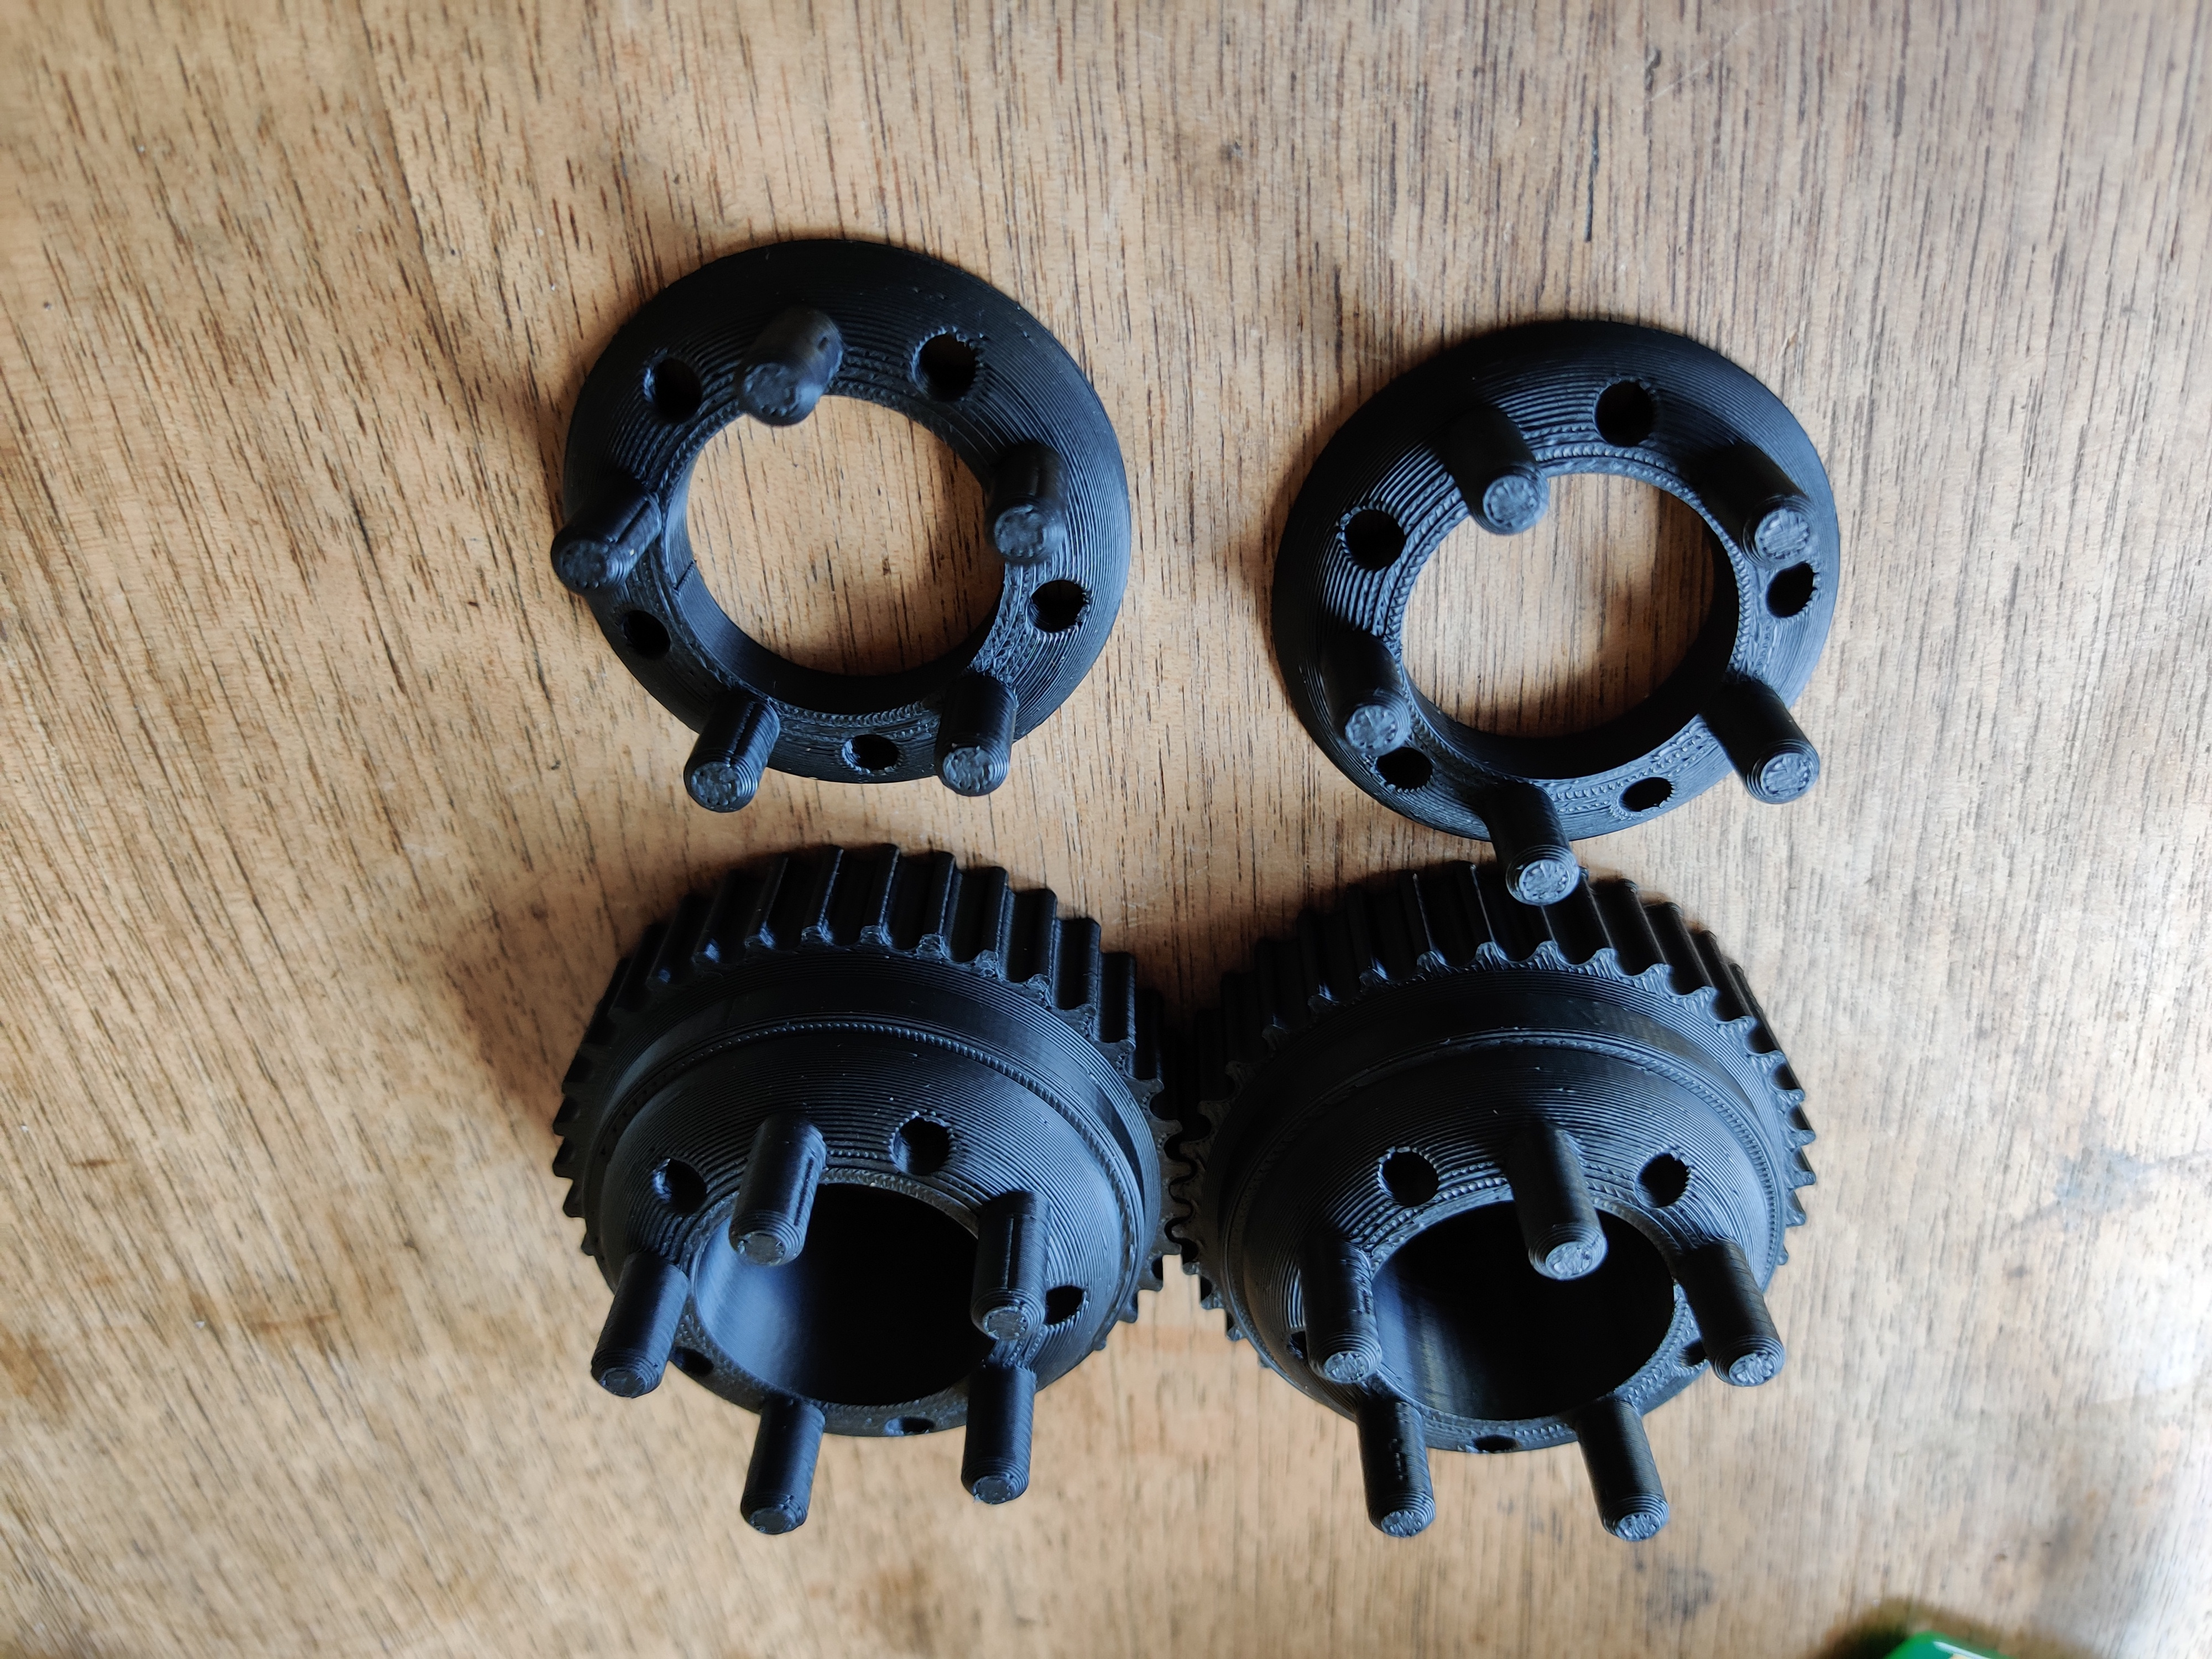
\includegraphics[angle=180, width=.49\textwidth]{Footage/Pictures/Wheel pulley v2.jpg}
			}
			\subcaptionbox{Zustand der Druckteile nach einigen Testfahrten.\label{subfig:printed pulleys after test driving}}[.49\textwidth][r]{
				\includegraphics[width=.49\textwidth]{Footage/Pictures/Wheel pulley v1.jpg}
			}
			\caption[Vergleich der gedruckten Zahn- und Konterscheiben vor und nach mehreren Testfahrten]{(a) Die finale und zum Zeitpunkt des Verfassens dieses Dokumentes noch verbaute Version. (b) Der Zustand des ersten funktionalen Prototypes nach etwa~\qty{100}{\kilo\metre} Testfahrt. Neben zu erwartender Verschmutzung sei insbesondere auf das Fehlen der Führungsstifte zu achten. Das Zahnprofil und die Komponenten als ganze weisen darüber hinaus jedoch keinerlei Anzeichen von Materialversagen auf.}
			\label{fig:comparison printed parts used unused}
		\end{figure}

	\section{Kosten}\label{sec:cost}
		Eine Aufstellung der Einzelkosten findet sich in \cref{tab:costs}.
		Die mit ``*'' gekennzeichneten Posten konnten im Rahmen des Projektes eingespart werden und sind mit Schätzwerten angegeben.
		Herstellung ohne Einsparmöglichkeit betrüge demnach \(\approx \dEUR{458,78}\).

		Das im Rahmen dieses Projektes hergestellte Antriebssystem lag mit \dEUR{264,75} gut unterhalb des fest gesetzten Preisrahmens von \dEUR{300} und mit rund \qty{58}{\percent} deutlich unterhalb der geschätzten Kosten von \dEUR{458,78}.
		Dies konnte allerdings nur realisiert werden, indem bereits vorhandene Aluminiumhalbzeuge genutzt und von einfacher und allem voran kostenfreier Möglichkeit des FDM-Drucks und der CNC-Fräsbearbeitung Gebrauch gemacht wurde.
		Das Kostenniveau extern gefertigter Druckteile wäre zwar mit \dEUR{23,03} als vergleichsweise moderat zu beschreiben, um unterhalb der Preisobergrenze zu bleiben war die Ersparnis der Fertigungs- und Materialkosten der Motorhalterung von \dEUR{170} jedoch maßgeblich\footnote{\hspace{1mm}Kostenvoranschläge für Druck- und Frästeile wurden jeweils unter online \url{www.pcbway.com} eingeholt.}.
		\newpage
		\begin{table}[ht!]
			\caption[Kostenaufstellung der Einzelteile]{Kostenaufstellung der Einzelteile. Da nicht alle Teile gekauft werden mussten, sind, wo zutreffend, Schätzwerte angegeben und mit ``*'' gekennzeichnet.}%
			\label{tab:costs}
			\centering
			\begin{threeparttable}
				\begin{tabular}{lp{1cm}r}
					\toprule
					Teil											&& Kosten\\
					\midrule
					Druckteile\tnote{a}								&& *\dEUR{23,03}\\
					\hspace{5mm}Nur Material						&& \dEUR{0,86}\\
					Motorhalterungen\tnote{a}						&& *\dEUR{170}\\
					% \hspace{5mm}Nur Halbzeug						&& *\dEUR{17,67}\\
					Motoren											&& \dEUR{177}\\
					Schrauben										&& *\dEUR{3}\\
					Steckverbinder									&& \dEUR{2}\\
					Rollen\tnote{b}									&& \dEUR{34,75}\\
					Zahnriemen										&& \dEUR{29,4}\\
					Zahnriemenscheiben								&& \dEUR{19,6}\\
																	&&\\
					\textbf{Gesamt}									&& \dEUR{264,75}\\
																	&& *\dEUR{458,78}\\
					\bottomrule
				\end{tabular}
				\begin{tablenotes}\footnotesize
					\item[a]	Fertigungsangebot inklusive Material.
					\item[b]	Preis für zwei Rollen.
				\end{tablenotes}
			\end{threeparttable}
		\end{table}